% ----------------------------------------------------------
% Introdução
% ----------------------------------------------------------
\chapter{Introdução}

\section{Objetivos}

O presente trabalho tem como objetivo geral desenvolver o \textit{SyncCarreira}, um \textit{software} proprietário do tipo \textit{SaaS} (\textit{Software as a Service}) destinado à automação e gestão de processos de orientação vocacional em instituições de ensino. A plataforma visa otimizar o fluxo de trabalho de psicólogos escolares, substituindo os métodos manuais de aplicação e correção de testes por um sistema digital integrado, e, simultaneamente, proporcionar aos alunos do ensino médio uma experiência mais interativa e acessível para a realização dos testes, consulta de seu histórico e acompanhamento profissional contínuo.

\subsection{Objetivos Específicos}

Para alcançar o propósito central, o projeto se desdobra nos seguintes objetivos específicos: automatizar a aplicação e correção de testes vocacionais por meio do desenvolvimento de um módulo digital que elimine a necessidade de processos manuais com papel e caneta, reduzindo a margem de erro humano e agilizando a obtenção dos resultados; possibilitar a customização de testes pela equipe de psicologia, implementando funcionalidades que permitam aos profissionais criar novos testes vocacionais, adaptar perguntas existentes e configurar baterias de avaliação personalizadas de acordo com as necessidades específicas de cada aluno ou turma; centralizar e digitalizar registros por meio da criação de um banco de dados centralizado e escalável para armazenar, de forma segura e organizada, o perfil dos alunos, todo o histórico de seus resultados e o \textit{feedback} registrado sobre cada teste realizado; implementar funcionalidades de gestão e análise que forneçam à equipe de psicologia ferramentas para administração de alunos, agendamento de sessões de acompanhamento e análise de dados, permitindo o reconhecimento de padrões e um acompanhamento mais qualificado dos estudantes; promover a reflexão do aluno sobre seus resultados por meio do desenvolvimento de um mecanismo que, ao final de cada teste, permita ao estudante registrar sua concordância ou não com os resultados obtidos, incentivando a autoanálise e gerando insumos valiosos para as sessões de acompanhamento com o psicólogo; e, por fim, garantir a customização e escalabilidade da plataforma, estruturando-a para que possa atender a múltiplas turmas e instituições sem perda de \textit{performance}, utilizando infraestrutura em nuvem.

\section{Problema e Solução Proposta}

A plataforma \textit{SyncCarreira} atua na automação e otimização dos processos de orientação vocacional para estudantes do Ensino Médio, oferecendo uma jornada personalizada e ferramentas especializadas que conferem ao sistema um diferencial competitivo frente às soluções convencionais disponíveis no mercado. O trabalho de orientação vocacional é complexo, envolvendo diversos testes que podem ser aplicados aos estudantes para ajudá-los num momento que pode ser difícil para muitos deles: a escolha da carreira que seguirão por muitos anos de suas vidas.

O grande desafio da orientação vocacional atual é que ela ainda depende, em grande parte, de processos manuais. Os psicólogos utilizam diversos testes e inventários para auxiliar os estudantes, mas como essas ferramentas são aplicadas em papel, o profissional precisa analisar e tabular os resultados de cada aluno um por um. O \textit{SyncCarreira} surge como uma solução para simplificar esse fluxo, permitindo que os psicólogos otimizem seu tempo e foquem no que é essencial: o acompanhamento terapêutico e as conversas com os estudantes, automatizando as tarefas burocráticas e repetitivas.

A aplicação possui dois tipos de perfis: psicólogos e estudantes, cada um com suas respectivas informações de cadastro e acessos. O perfil psicólogo é o que possui maior controle e ingerência sobre o que acontece na aplicação. Ele tem acesso ao histórico e resultados de todos os estudantes que estão associados a ele, tem controle sobre quais testes são enviados a quais estudantes, pode alterar, criar e excluir testes, além de agendar horários e enviar notificações para que os estudantes selecionados executem os testes. Em suma, o perfil do psicólogo define o fluxo da orientação vocacional que é aplicado dentro do aplicativo. Por outro lado, o perfil estudante tem acesso apenas ao seu próprio histórico de resultados nos testes e suas avaliações psicológicas, garantindo o sigilo necessário a esses usuários.

Haverá a opção de alterar o idioma da aplicação para o inglês para uma possível implementação do sistema em escolas e outras instituições bilíngues. Adicionalmente, será possível para os psicólogos cadastrarem perfis de tipos de personalidades, que serão associadas aos estudantes com base nos resultados de seus testes e orientações vocacionais. Essas informações poderão ser agrupadas em relatórios, para que se possa ter uma visão geral da orientação.

Tanto o perfil psicólogo quanto o perfil estudante poderão enviar \textit{feedbacks} personalizados, para que haja uma comunicação efetiva entre os usuários mesmo quando não for possível o encontro presencial para orientação. O perfil de estudante poderá personalizar seus interesses prévios, para que se possa ter uma noção geral inicial de tendências a carreiras ou áreas de atuação. Agendamentos de testes e de encontros poderão ser visualizados pelos perfis e podem ser aceitos ou recusados, conforme a necessidade de horários de cada usuário.

Em suma, o \textit{SyncCarreira} traz benefícios tanto para os estudantes em fase de escolha de carreira quanto para os psicólogos, facilitando a comunicação, automatizando processos, ajudando os profissionais da área da Psicologia a se concentrarem mais nas partes fundamentais do trabalho e menos nas partes burocráticas, contribuindo para o sucesso de todos envolvidos.

\section{Justificativa}

A relevância do projeto \textit{SyncCarreira} fundamenta-se na urgente necessidade de modernização tecnológica em um setor vital para o desenvolvimento estudantil: a orientação vocacional. Atualmente, a persistência de métodos manuais baseados em suporte físico (papel e caneta) cria um gargalo operacional que limita a atuação do psicólogo escolar e compromete a agilidade do processo. A automação proposta por este trabalho justifica-se, primordialmente, pela otimização da eficiência operacional, uma vez que a digitalização da aplicação e correção de testes elimina tarefas burocráticas e repetitivas. Ao reduzir a margem de erro humano e acelerar a entrega de resultados, a solução permite que o profissional direcione seu foco para a dimensão analítica e terapêutica, oferecendo um suporte mais estratégico e humanizado ao orientando.

Sob a ótica social e educacional, o desenvolvimento desta plataforma responde aos desafios enfrentados por jovens em fase pré-vestibular, período de intensa pressão psíquica e escolhas determinantes. Ao oferecer uma interface interativa e acessível, o \textit{SyncCarreira} promove maior engajamento dos estudantes, alinhando a prática da psicologia escolar à realidade digital da geração atual. Além disso, a centralização do histórico de resultados em um banco de dados seguro garante a continuidade do acompanhamento profissional, transformando a orientação vocacional em uma jornada documentada e longitudinal, o que confere maior robustez ao processo de autoconhecimento do aluno.

Do ponto de vista técnico e institucional, a importância do \textit{software} estende-se pela sua arquitetura como modelo \textit{Software as a Service} (\textit{SaaS}) e sua escalabilidade em nuvem. Tais características conferem ao projeto uma extensão significativa, permitindo que instituições de diferentes portes e contextos --- incluindo escolas bilíngues, dada a funcionalidade de internacionalização --- adotem o sistema com baixo custo de infraestrutura inicial. A capacidade de customização de testes e a geração de relatórios gerenciais não apenas organizam a gestão de informações sensíveis, em conformidade com o sigilo profissional, mas também fornecem insumos valiosos para que as instituições identifiquem padrões de interesse e aprimorem suas diretrizes pedagógicas.

Para compreender a gravidade do problema gerado por escolhas profissionais precipitadas, os microdados do Instituto Nacional de Estudos e Pesquisas Educacionais Anísio Teixeira (INEP) revelam um cenário alarmante de abandono. Acompanhando a trajetória dos estudantes ingressantes no Ensino Superior no ano de 2015, nos gráficos abaixo \cite{inep2026}:

\begin{figure}[H]
    \centering
    \caption{Gráfico 1 -- Trajetória histórica de estudantes do Ensino Superior.}
    \label{fig_grafico_inep1}
    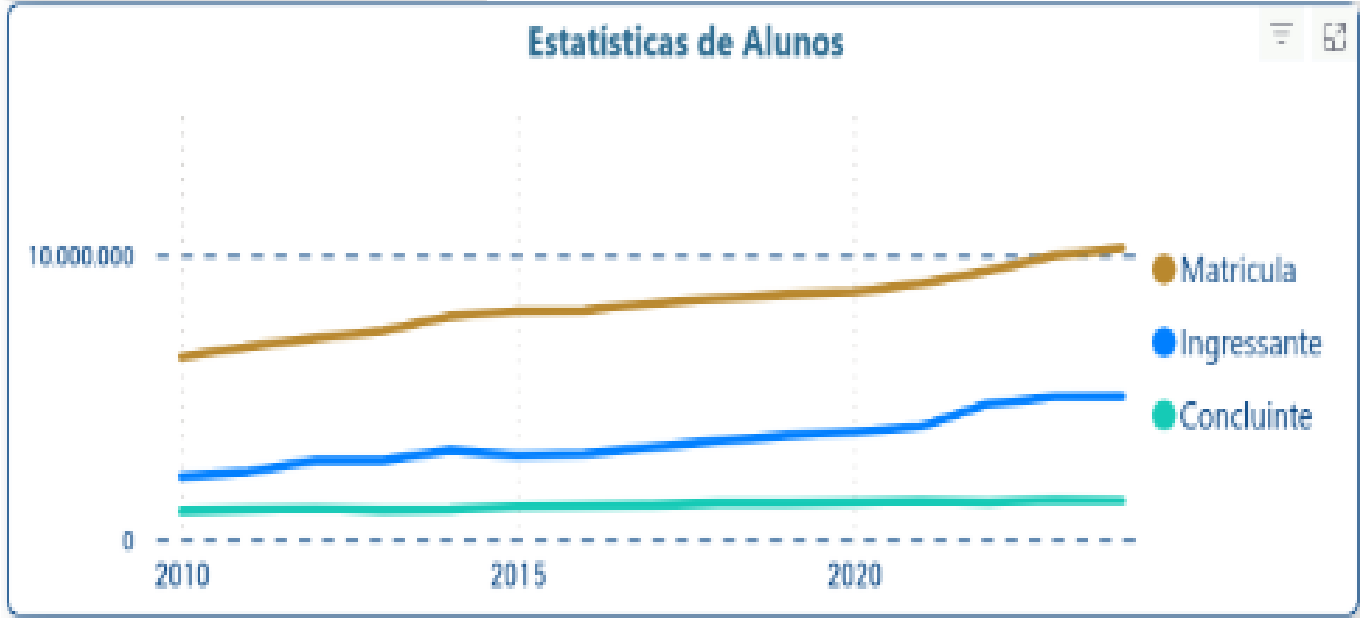
\includegraphics[width=0.85\textwidth]{img/graf-1-trajetoria-historica-ensino-superior.png}
    \legend{Fonte: \citeonline{inep2026}.}
\end{figure}

\begin{figure}[H]
    \centering
    \caption{Gráfico 2 -- Taxa de conclusão anual no Ensino Superior dos ingressantes de 2015.}
    \label{fig_grafico_inep2}
    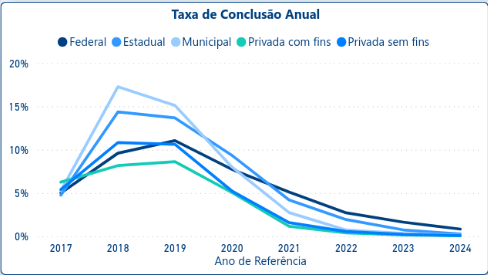
\includegraphics[width=0.85\textwidth]{img/graf-2-taxa-conclusao-anual.png}
    \legend{Fonte: \citeonline{inep2026}.}
\end{figure}

\begin{figure}[H]
    \centering
    \caption{Gráfico 3 -- Taxa de desistência anual acumulada no Ensino Superior (Coorte de Ingressantes em 2015).}
    \label{fig_grafico_inep3}
    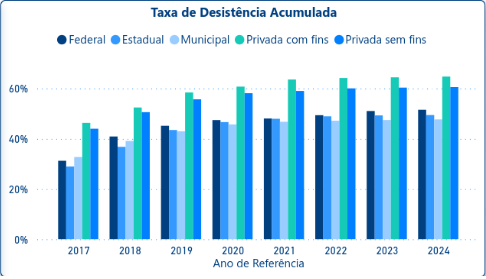
\includegraphics[width=0.85\textwidth]{img/graf-3-taxa-desistencia-acumulada.png}
    \legend{Fonte: \citeonline{inep2026}.}
\end{figure}

Os números apresentados evidenciam que grande parte do problema da evasão universitária, que gera desperdício de tempo para o aluno e perda financeira para o sistema educacional, tem raiz na transição do Ensino Médio para o Superior. A escolha baseada em impulso, pressão externa ou falta de autoconhecimento resulta em frustrações futuras.

No ecossistema escolar, a psicóloga é a profissional capacitada para mitigar esse risco através da Orientação Vocacional. Entretanto, ao ficarem restritas a processos analógicos (como a aplicação de testes em papel e a tabulação de planilhas de resultados), as profissionais deixam de aplicar sua principal especialidade: a interpretação psicológica e a escuta ativa do aluno. Os dados mostram que a falta dessa orientação qualificada deságua nas estatísticas de evasão nos anos seguintes.

\section{Análise da Concorrência}

Para o desenvolvimento estrutural e visual do sistema, foi realizado um estudo de \textit{benchmarking} com o intuito de identificar as principais soluções disponíveis no mercado que tangenciam o escopo de testes vocacionais e mapeamento de perfil. Compreender o cenário atual do mercado é uma etapa fundamental para o desenvolvimento e o posicionamento de qualquer solução tecnológica. Conforme apontam \citeonline{kotler2012}, o planejamento de estratégias eficazes exige que a organização pesquise e compreenda o mais profundamente possível a atuação dos seus concorrentes.

A análise a seguir foca em quatro plataformas amplamente utilizadas pelo público jovem --- 16Personalities, Descomplica, CareerExplorer e Qual Carreira --- destacando seus pontos fortes e as lacunas que a aplicação desenvolvida neste projeto se propõe a preencher no contexto escolar.

\subsection{16 Personalities}

O 16Personalities é uma plataforma global de mapeamento de personalidade baseada na teoria de traços e nos conceitos de Myers-Briggs. Embora não seja estritamente um teste vocacional voltado para a escolha de carreiras, é uma ferramenta amplamente utilizada por jovens em fase de autodescoberta.

A plataforma destaca-se excepcionalmente pela sua Interface de Usuário (UI) e Experiência do Usuário (UX). A utilização de uma escala de concordância visual (Escala Likert) torna o preenchimento fluido, rápido e menos cansativo para o jovem. Além disso, a devolutiva dos resultados é gamificada, utilizando avatares e descrições de fácil compreensão, gerando alta identificação.

\begin{figure}[htb]
    \centering
    \caption{Interface do teste de personalidade da plataforma 16Personalities.}
    \label{fig_16personalities}
    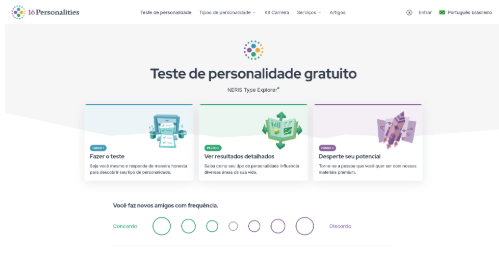
\includegraphics[width=0.80\textwidth]{img/fig-1-16personalities.png}
    \legend{Fonte: 16PERSONALITIES (2026).}
\end{figure}

\subsection{Descomplica}

O Descomplica é uma das maiores plataformas de educação \textit{online} do Brasil, com forte atuação na preparação para o ENEM e grandes vestibulares. Como parte de sua jornada de atração e engajamento, a plataforma disponibiliza testes vocacionais rápidos para os estudantes.

A principal vantagem é a acessibilidade e a linguagem altamente alinhada à realidade do estudante do Ensino Médio brasileiro. A plataforma consegue vincular de forma imediata o resultado de um teste de perfil com opções de cursos superiores reais e tendências de mercado, facilitando a visualização dos próximos passos acadêmicos do aluno.

\begin{figure}[htb]
    \centering
    \caption{Interface do teste vocacional da plataforma Descomplica.}
    \label{fig_descomplica}
    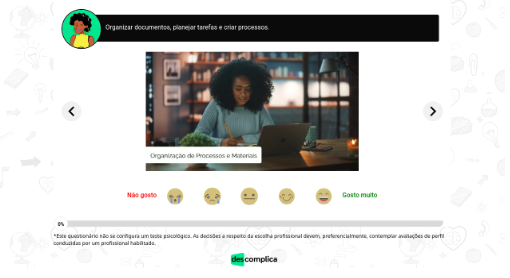
\includegraphics[width=0.80\textwidth]{img/fig-2-descomplica.png}
    \legend{Fonte: DESCOMPLICA (2026).}
\end{figure}

\subsection{Qual Carreira}

A plataforma Qual Carreira é uma ferramenta \textit{web} focada em orientação vocacional, auxiliando milhares de usuários a filtrar as centenas de graduações existentes e sugerindo aquelas que melhor se adequam à sua personalidade e objetivos. Além disso, funciona como um portal de conteúdo e notícias, mantendo seu público, composto majoritariamente por estudantes e universitários, sempre informado sobre temas essenciais, como calendários de provas e atualizações no sistema educacional brasileiro.

\begin{figure}[htb]
    \centering
    \caption{Interface do teste vocacional da plataforma Qual Carreira.}
    \label{fig_qualcarreira}
    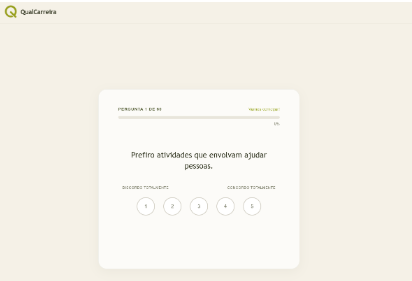
\includegraphics[width=0.80\textwidth]{img/fig-3-qualcarreira.png}
    \legend{Fonte: QUALCARREIRA (2026).}
\end{figure}

\subsection{CareerExplorer}

A plataforma \textit{web} CareerExplorer é uma referência em sistemas de orientação de carreira. Utiliza uma interface moderna e altamente atrativa, gerando relatórios personalizados para seus usuários. Além disso, a ferramenta sugere certificações e cursos alinhados aos objetivos individuais, tendo como um de seus grandes diferenciais a alta taxa de personalização. Seu foco abrange um amplo espectro de usuários, desde universidades e jovens recém-saídos do ensino médio, até jovens adultos em dúvida sobre a graduação e profissionais que buscam uma transição de carreira.

\begin{figure}[htb]
    \centering
    \caption{Interface do teste vocacional da plataforma CareerExplorer.}
    \label{fig_careerexplorer}
    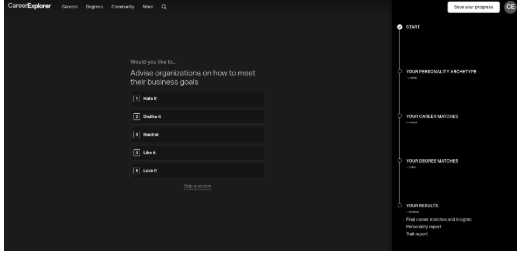
\includegraphics[width=0.80\textwidth]{img/fig-4-careerexplorer.png}
    \legend{Fonte: CARREREXPLORER (2026).}
\end{figure}

\subsection{Comparativo}

Abaixo, o \autoref{quadro-comparativo} resume as funcionalidades da plataforma frente às soluções de mercado:

\begin{table}[htb]
\ABNTEXfontereduzida
\caption[Comparação de Recursos entre os Projetos]{Comparação de Recursos entre os Projetos.}
\label{quadro-comparativo}
\begin{tabular}{|p{4cm}|c|c|c|c|c|}
\hline
\textbf{Funcionalidades Principais} & \textbf{16pers.} & \textbf{Descomplica} & \textbf{Qual Carreira} & \textbf{CareerExplorer} & \textbf{SyncCarreira} \\
\hline
Login (Aluno/Psicóloga) & $\checkmark$ & $\checkmark$ &  & $\checkmark$ & $\checkmark$ \\
\hline
Painel da Psicóloga &  &  &  &  & $\checkmark$ \\
\hline
Dashboard do Aluno &  &  &  &  & $\checkmark$ \\
\hline
Relatórios (Aluno/Turma) & $\checkmark$ & $\checkmark$ &  & $\checkmark$ & $\checkmark$ \\
\hline
Histórico de Testes & $\checkmark$ & $\checkmark$ &  & $\checkmark$ & $\checkmark$ \\
\hline
Feedback Automatizado & $\checkmark$ & $\checkmark$ & $\checkmark$ & $\checkmark$ & $\checkmark$ \\
\hline
Feedback da Psicóloga &  & $\checkmark$ &  &  & $\checkmark$ \\
\hline
Gestão de Agendamentos &  &  &  &  & $\checkmark$ \\
\hline
Cadastro de Testes Próprios &  &  &  &  & $\checkmark$ \\
\hline
Multi-idioma (Inglês) & $\checkmark$ &  &  & $\checkmark$ & $\checkmark$ \\
\hline
\end{tabular}
\legend{Fonte: Autores (2026).}
\end{table}
